% !TEX root = main.tex
\section{Kết quả thực nghiệm}\label{sec:exp}

\subsection{Cấu hình thực nghiệm}\label{sec:exp:setup}

\textbf{Môi trường chạy.} Toàn bộ thực nghiệm chạy trên một máy tính xách tay chỉ dùng CPU; cấu hình phần cứng và phần
mềm được liệt kê ở Bảng~\ref{tab:env}. Mã nguồn viết bằng Python, phần lõi tìm kiếm dùng \texttt{heapq} trên cấu trúc
CSR (thư viện NetworkX chỉ dùng để đối chiếu kết quả trong kiểm thử đơn vị).

\begin{table}[H]
\centering\small
\renewcommand{\arraystretch}{1.2}
\caption{Môi trường phần cứng và phần mềm.}
\label{tab:env}
\begin{tabularx}{\linewidth}{>{\raggedright\arraybackslash}p{4.2cm}X}
\toprule
\textbf{Thành phần} & \textbf{Cấu hình} \\
\midrule
Phần cứng & Laptop Intel 16 luồng, chỉ CPU (không dùng GPU) \\
Hệ điều hành & Windows 11; kiểm tra lại trong container Docker Linux \\
Ngôn ngữ & Python 3.13 \\
Dữ liệu bản đồ & OSMnx 2.1, GeoPandas, Shapely \\
Tính toán số & NumPy, SciPy, Numba 0.68 \\
Học tăng cường & Gymnasium 1.4, Stable-Baselines3 / sb3-contrib 2.9, PyTorch 2.10 \\
Trực quan, giao diện & Matplotlib, Seaborn, Streamlit, Folium, pydeck \\
Kiểm thử & pytest (55 kiểm thử đơn vị) \\
\bottomrule
\end{tabularx}
\end{table}

\textbf{Cách chọn tham số và số lần lặp.} Seed toàn cục là \Seed{}; mọi seed con (nhiễu của từng truy vấn, môi trường RL,
khởi tạo mạng) được dẫn xuất tất định từ seed này. Các tham số mô phỏng (biên độ cao điểm, độ nhạy loại đường, hệ số
hướng, mức nhiễu) được chọn theo hiểu biết chung về giao thông đô thị và hiệu chỉnh sơ bộ để vận tốc trung bình hợp lý; các
tham số thuật toán (bán kính quan sát, ngưỡng lười, số điểm mốc, hệ số thưởng) được thử sơ bộ trên tập kiểm định và
\emph{cố định trước khi chạy tập kiểm tra}. Mỗi biến thể RL được huấn luyện với \RlNSeeds{} seed; ngân sách số bước từ 60
nghìn (biến thể lai) tới 1 triệu (định hình ctg), xem Bảng~\ref{tab:tab_rl_seeds}. Chính sách được đánh giá định kỳ trên 100
truy vấn kiểm định và lưu checkpoint có điểm cao nhất theo
\begin{equation}
\text{score} = \text{tỉ lệ tới đích} - 0{,}002\times\text{regret}\ (\%),
\label{eq:score}
\end{equation}
và bảng chính dùng seed tốt nhất theo tập kiểm định (không chọn theo tập kiểm tra). Thời gian tính được đo \emph{đơn luồng}
(một tiến trình, tuần tự, sau khi làm nóng bộ nhớ đệm và JIT) trên \RuntimeNQ{} truy vấn kiểm tra. Bảng tham số đầy đủ ở
Phụ lục (Bảng~\ref{tab:tab_config}).

\subsection{Phương pháp baseline để so sánh}\label{sec:exp:baseline}

\begin{itemize}
    \item \textbf{Dijkstra ngắn nhất}~\cite{dijkstra1959}: tuyến ngắn nhất theo chiều dài. Ưu điểm: đơn giản, rất nhanh;
    nhược điểm: không biết giờ cao điểm. Đây là mốc ``không dùng thông tin giao thông''.
    \item \textbf{A* theo thời gian tự do}~\cite{hart1968}: tuyến nhanh nhất khi đường thông thoáng; biết loại đường nhưng không
    biết ùn tắc theo giờ.
    \item \textbf{Plan-once TD-A*}~\cite{dreyfus1969,kaufman1993}: tối ưu theo dự báo lúc xuất phát, không thích nghi trong khi đi.
    \item \textbf{Oracle TD-A*}: chạy TD-A* trên chính $V_{\text{real}}$ (biết trước tương lai) --- không khả thi trong thực tế,
    chỉ dùng làm cận dưới để tính regret \eqref{eq:regret}.
    \item \textbf{Tham lam cục bộ}: chọn cạnh có cosin hướng đích lớn nhất, phạt nút đã thăm; dùng \emph{cùng} quan sát với RL
    cục bộ nên là mốc dưới tự nhiên cho các chính sách RL.
    \item \textbf{Replan TD-A*}: baseline thích nghi chính, dùng để đánh giá các phương pháp mới (replan lười, D* Lite, GCN, RL lai).
\end{itemize}

\subsection{Các bộ dữ liệu sử dụng}\label{sec:exp:data}

\textbf{Dữ liệu thực (real-world).} Mạng đường OpenStreetMap của quận Hà Đông cộng vùng đệm 500~m: \NNodes{} nút,
\NEdges{} cạnh, \TotalKm{} km (Bảng~\ref{tab:tab_graph_groups}); toạ độ các điểm nóng lấy từ Nominatim.

\textbf{Dữ liệu tổng hợp (synthetic).} Vận tốc 24 khung giờ được mô phỏng theo Mục~\ref{sec:method:speed}; môi trường thực
theo Mục~\ref{sec:method:noise}. Tập truy vấn gồm 1000 truy vấn được sinh với các ràng buộc: khoảng cách chim bay giữa hai
điểm ít nhất 1 km, giờ xuất phát lấy mẫu có trọng số ưu tiên cao điểm, mức nhiễu $\sigma\in\{0{,}05;0{,}15;0{,}30\}$, số sự
cố $\{0,1,2,3\}$ với xác suất $0{,}35/0{,}30/0{,}20/0{,}15$. Tập được chia \NTrain/\NVal/\NTest{} (huấn luyện/kiểm
định/kiểm tra) \emph{theo cặp điểm đi--đến}, không có cặp nào xuất hiện ở hai tập; các cạnh có sự cố trong tập kiểm tra
chưa từng xuất hiện trong tập huấn luyện. Tập kiểm tra có khoảng cách chim bay trung bình \TestMeanDistKm{} km và trung bình
\TestMeanInc{} sự cố mỗi truy vấn.

\textbf{Hai bộ sự cố trên cùng truy vấn.} Mỗi truy vấn kiểm tra có hai bộ sự cố cùng số lượng, cùng thời điểm và cùng mức
độ, chỉ khác vị trí: \emph{tập chính} đặt sự cố ngẫu nhiên trên hành lang 600~m quanh đoạn thẳng nối hai điểm, không thiên
vị phương pháp nào; \emph{tập stress} đặt sự cố lên tuyến dự kiến của plan-once với xác suất \StressProb, cố ý gây bất lợi
cho plan-once để kiểm tra sức chịu đựng. GCN được huấn luyện trên các ``ngày'' mô phỏng có seed riêng, độc lập với mọi tập
truy vấn.

\subsection{Các tiêu chí đánh giá}\label{sec:exp:metrics}

\begin{itemize}
    \item \textbf{Thời gian di chuyển thực tế} (trung bình, trung vị, phân vị 90\%): mục tiêu trực tiếp của người lái;
    phân vị 90\% phản ánh độ tin cậy.
    \item \textbf{Regret so với oracle} \eqref{eq:regret}: chuẩn hoá theo độ khó của từng truy vấn, cho phép so sánh giữa
    chuyến ngắn và chuyến dài.
    \item \textbf{Tỉ lệ tới đích}: chính sách RL chọn từng cạnh có thể không tới đích trong giới hạn số bước; thời gian và
    regret chỉ tính trên các chuyến tới đích nên luôn phải đọc kèm tỉ lệ này.
    \item \textbf{Số nút mở rộng và thời gian tính đơn luồng}: chi phí tính toán, lần lượt độc lập phần cứng và thực tế.
    \item \textbf{Ý nghĩa thống kê.} Vì mọi phương pháp chạy trên cùng truy vấn, chúng tôi so sánh \emph{ghép cặp}. Với hiệu
    $D_i=T^A_i-T^B_i$ trên $n$ truy vấn, khoảng tin cậy bootstrap~\cite{efron1993} 95\% của $\bar{D}$ là
    \begin{equation}
    \mathrm{CI}_{95\%} = \Bigl[\widehat{q}_{0.025}\bigl(\bar{D}^{\ast(b)}\bigr),\; \widehat{q}_{0.975}\bigl(\bar{D}^{\ast(b)}\bigr)\Bigr]_{b=1}^{B},
    \label{eq:bootstrap}
    \end{equation}
    với $\bar{D}^{\ast(b)}$ là trung bình của mẫu lấy lại có hoàn lại thứ $b$ và $B=5000$. Kiểm định Wilcoxon
    signed-rank~\cite{wilcoxon1945} dùng thống kê
    \begin{equation}
    W = \sum_{i:\,D_i\neq 0} \operatorname{sgn}(D_i)\, R_i,
    \label{eq:wilcoxon}
    \end{equation}
    trong đó $R_i$ là hạng của $|D_i|$; kiểm định không giả định phân phối chuẩn, phù hợp với phân phối lệch của regret.
    \item \textbf{Riêng cho từng thí nghiệm.} Dự báo GCN dùng sai số căn quân phương trên các cạnh chưa quan sát:
    \begin{equation}
    \mathrm{RMSE} = \sqrt{\frac{1}{|U|}\sum_{e\in U}\bigl(\hat{r}_e - r_e\bigr)^2},
    \label{eq:rmse}
    \end{equation}
    với $U$ là tập cạnh không có quan sát. Định tuyến P90 dùng trung bình và phân vị 90\% trên 100 kịch bản độc lập; chọn
    giờ xuất phát dùng chi phí \eqref{eq:departure}; mô phỏng nhiều xe dùng thời gian đi trung bình khi có tải \eqref{eq:bpr}.
\end{itemize}

\subsection{Phân tích kết quả}\label{sec:exp:results}

\subsubsection{Kết quả tổng hợp: tìm kiếm, tái lập kế hoạch, dự báo}

Bảng~\ref{tab:tab_main_classic} và Hình~\ref{fig:box} trình bày kết quả trên tập kiểm tra chính (\NTest{} truy vấn). Kết
quả xác nhận giả thuyết H1: chỉ riêng việc tính đến sự phụ thuộc thời gian đã giảm regret trung bình từ \DijRegret\% (Dijkstra
ngắn nhất) và \FfRegret\% (A* theo thời gian tự do) xuống \PoRegret\% (plan-once TD-A*). Tái lập kế hoạch tiếp tục đưa
regret về \RpRegret\%; replan lười đạt \RpLazyRegret\% và D* Lite đạt \RpDstarRegret\%. Phương pháp tốt nhất là replan kết hợp
dự báo GCN với regret \RpGnnRegret\%. Ở chế độ lập kế hoạch một lần, sử dụng cảm biến mà không lan truyền cho
\PoSenRegret\%, còn khi lan truyền bằng GCN cho \PoGnnRegret\%. Định tuyến P90 cho \RiskRegret\%. Mọi phương pháp tìm kiếm
đều tới đích 100\%.

\begin{table}[!htbp]
\centering
\small
\caption{Kết quả các phương pháp tìm kiếm và dự báo trên tập kiểm tra chính (200 truy vấn, sự cố đặt ngẫu nhiên) trong môi trường thực; regret tính so với oracle.}
\label{tab:tab_main_classic}
\begin{adjustbox}{max width=\linewidth}
\begin{tabular}{lrrrrrrrr}
\toprule
Phương pháp & Tới đích (\%) & TB (phút) & Trung vị & P90 & Regret TB (\%) & Regret TV (\%) & Regret P90 (\%) & Dài (km) \\
\midrule
Dijkstra (ngắn nhất) & 100{,}00 & 19{,}01 & 16{,}05 & 33{,}12 & 11{,}03 & 7{,}63 & 26{,}73 & 6{,}26 \\
A* (thời gian tự do) & 100{,}00 & 18{,}33 & 14{,}96 & 31{,}42 & 5{,}21 & 0{,}19 & 16{,}49 & 6{,}64 \\
Plan-once TD-A* & 100{,}00 & 17{,}51 & 14{,}51 & 31{,}05 & 1{,}29 & 0{,}00 & 4{,}64 & 6{,}62 \\
Plan-once + cảm biến & 100{,}00 & 17{,}43 & 14{,}51 & 30{,}89 & 0{,}92 & 0{,}00 & 2{,}85 & 6{,}60 \\
Plan-once + GCN & 100{,}00 & 17{,}39 & 14{,}47 & 31{,}04 & 0{,}59 & 0{,}00 & 1{,}22 & 6{,}58 \\
Định tuyến P90 & 100{,}00 & 17{,}53 & 14{,}62 & 31{,}08 & 1{,}47 & 0{,}00 & 4{,}75 & 6{,}63 \\
Replan TD-A* & 100{,}00 & 17{,}35 & 14{,}47 & 30{,}89 & 0{,}47 & 0{,}00 & 1{,}18 & 6{,}63 \\
Replan lười & 100{,}00 & 17{,}36 & 14{,}47 & 30{,}89 & 0{,}48 & 0{,}00 & 1{,}18 & 6{,}64 \\
Replan D* Lite & 100{,}00 & 17{,}37 & 14{,}47 & 31{,}04 & 0{,}44 & 0{,}00 & 1{,}44 & 6{,}62 \\
Replan + GCN & 100{,}00 & 17{,}31 & 14{,}47 & 31{,}04 & 0{,}19 & 0{,}00 & 0{,}01 & 6{,}61 \\
Oracle TD-A* & 100{,}00 & 17{,}26 & 14{,}47 & 30{,}89 & 0{,}00 & 0{,}00 & 0{,}00 & 6{,}64 \\
\bottomrule
\end{tabular}
\end{adjustbox}
\end{table}


\begin{figure}[H]
\centering
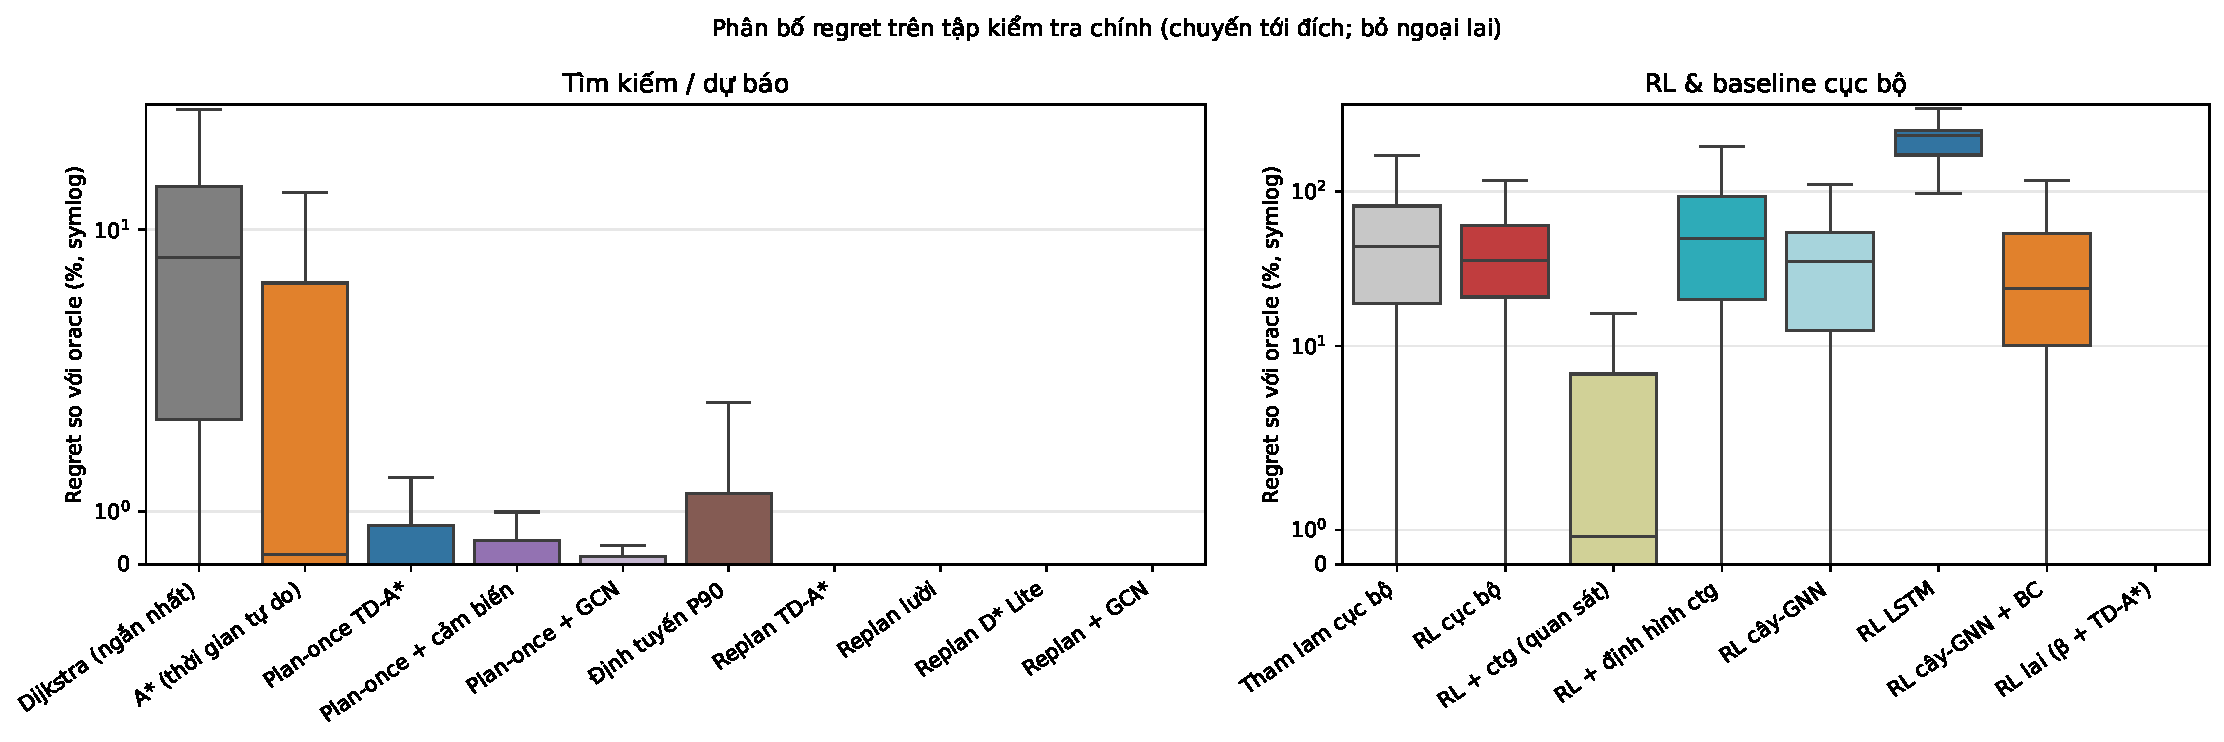
\includegraphics[width=\linewidth]{boxplot_methods.pdf}
\caption{Phân bố regret theo phương pháp trên tập kiểm tra chính (chuyến tới đích; trục tung dạng symlog).}
\label{fig:box}
\end{figure}

\textbf{Kiểm định thống kê} (Bảng~\ref{tab:tab_stat_tests}). Với mỗi cặp (A, B), chúng tôi báo cáo hiệu thời gian trung
bình $\bar{D}=\overline{T^A-T^B}$ (giá trị âm nghĩa là A nhanh hơn), khoảng tin cậy bootstrap 95\% \eqref{eq:bootstrap} và
giá trị $p$ của kiểm định Wilcoxon \eqref{eq:wilcoxon}:
\begin{itemize}
    \item Plan-once so với Dijkstra: $\bar{D}=\DiffPlanOnceDijkstraLength$ phút mỗi chuyến, khoảng tin cậy
    \CiPlanOnceDijkstraLength, $p$ \PPlanOnceDijkstraLength.
    \item Replan so với plan-once: $\bar{D}=\DiffReplanPlanOnce$ phút, khoảng tin cậy \CiReplanPlanOnce, $p$ \PReplanPlanOnce.
    \item Replan + GCN so với replan: $\bar{D}=\DiffReplanGnnReplan$ phút, khoảng tin cậy \CiReplanGnnReplan, $p$ \PReplanGnnReplan.
    \item Plan-once + GCN so với plan-once: $\bar{D}=\DiffPlanOnceGnnPlanOnce$ phút, khoảng tin cậy \CiPlanOnceGnnPlanOnce,
    $p$ \PPlanOnceGnnPlanOnce.
    \item Replan lười so với replan: $\bar{D}=\DiffReplanLazyReplan$ phút, khoảng tin cậy \CiReplanLazyReplan{} --- thực tế
    không khác biệt; D* Lite so với replan: $\bar{D}=\DiffReplanDstarReplan$ phút, khoảng tin cậy \CiReplanDstarReplan{} chứa 0.
    \item Định tuyến P90 so với plan-once: $\bar{D}=\DiffRiskPPlanOnce$ phút, khoảng tin cậy \CiRiskPPlanOnce, $p$
    \PRiskPPlanOnce{} --- định tuyến P90 hơi \emph{chậm hơn}.
\end{itemize}
Các khác biệt tính bằng phút là nhỏ vì phần lớn truy vấn không chịu ảnh hưởng của sự cố, nhưng nhất quán (khoảng tin cậy
không chứa 0) ở các cặp chính.

\begin{table}[!htbp]
\centering
\small
\caption{So sánh ghép cặp trên các truy vấn cả hai phương pháp cùng tới đích: khoảng tin cậy bootstrap 95\% của hiệu trung bình thời gian và kiểm định Wilcoxon signed-rank.}
\label{tab:tab_stat_tests}
\begin{adjustbox}{max width=\linewidth}
\begin{tabular}{lrrrrrrr}
\toprule
Cặp (A − B) & n & Hiệu TB (phút) & CI 95\% thấp & CI 95\% cao & Hiệu TB (\%) & A tốt hơn (\%) & p (Wilcoxon) \\
\midrule
Plan-once TD-A* − Dijkstra (ngắn nhất) & 200 & -1{,}499 & -1{,}738 & -1{,}270 & -7{,}974 & 78{,}000 & $<10^{-4}$ \\
Replan TD-A* − Plan-once TD-A* & 200 & -0{,}159 & -0{,}250 & -0{,}084 & -0{,}726 & 36{,}500 & $<10^{-4}$ \\
Oracle TD-A* − Replan TD-A* & 200 & -0{,}090 & -0{,}142 & -0{,}050 & -0{,}440 & 18{,}500 & $<10^{-4}$ \\
Replan lười − Replan TD-A* & 200 & 0{,}002 & 0{,}000 & 0{,}004 & 0{,}007 & 0{,}500 & 0{,}0687 \\
Replan D* Lite − Replan TD-A* & 200 & 0{,}015 & -0{,}036 & 0{,}077 & -0{,}020 & 3{,}500 & 0{,}3037 \\
Replan + GCN − Replan TD-A* & 200 & -0{,}048 & -0{,}105 & 0{,}005 & -0{,}250 & 10{,}500 & 0{,}0186 \\
Plan-once + cảm biến − Plan-once TD-A* & 200 & -0{,}081 & -0{,}155 & -0{,}013 & -0{,}316 & 16{,}000 & 0{,}0297 \\
Plan-once + GCN − Plan-once TD-A* & 200 & -0{,}124 & -0{,}199 & -0{,}055 & -0{,}635 & 26{,}000 & $<10^{-4}$ \\
Plan-once + GCN − Plan-once + cảm biến & 200 & -0{,}043 & -0{,}093 & 0{,}008 & -0{,}308 & 21{,}500 & 0{,}0002 \\
Định tuyến P90 − Plan-once TD-A* & 200 & 0{,}015 & -0{,}010 & 0{,}038 & 0{,}188 & 6{,}000 & 0{,}0027 \\
RL lai (β + TD-A*) − Replan TD-A* & 200 & 0{,}013 & 0{,}004 & 0{,}025 & 0{,}082 & 0{,}000 & 0{,}0009 \\
RL cây-GNN + BC − Plan-once TD-A* & 154 & 5{,}527 & 4{,}473 & 6{,}798 & 35{,}788 & 3{,}896 & $<10^{-4}$ \\
RL + ctg (quan sát) − A* (thời gian tự do) & 200 & -0{,}001 & -0{,}079 & 0{,}063 & 0{,}096 & 7{,}000 & 0{,}0002 \\
\bottomrule
\end{tabular}
\end{adjustbox}
\end{table}


\subsubsection{Chi phí tính toán}

Bảng~\ref{tab:tab_runtime_single} và Hình~\ref{fig:exp} so sánh chi phí tính toán đơn luồng. A* giảm \AstarReduction\% số nút
mở rộng so với Dijkstra. Với tìm kiếm phụ thuộc thời gian, heuristic chim bay chỉ giảm \TdAstarReduction\% so với TD-Dijkstra
vì phải chia cho $v_{\max}$ lớn (vận tốc tự do lớn nhất) trong khi vận tốc thực tế, nhất là giờ cao điểm, thấp hơn nhiều.
Heuristic cận dưới chính xác giảm \LbReduction\% (ít hơn heuristic chim bay \LbVsEuclid\%) nhưng tốn \LbPrep{} ms tiền xử lý
mỗi đích; ALT giảm \AltReduction\% với \AltPrep{} ms để tính heuristic mỗi truy vấn (tiền xử lý điểm mốc chỉ làm một lần).
TD-A* biên dịch Numba nhanh gấp \NumbaSpeedup{} lần bản Python với cùng số nút mở rộng. Replan tốn \RtRp{} ms mỗi chuyến
(\RpReplans{} lần tìm kiếm); replan lười nhanh gấp \LazySpeedup{} lần (\RpLazyReplans{} lần tìm kiếm); D* Lite nhanh gấp
\DstarSpeedup{} lần (\RpDstarExpanded{} nút mở rộng so với \RpExpanded{} của replan). Suy luận chính sách RL (PyTorch, từng
bước) tốn \RtRl{}--\RtRlTreeBc{} ms mỗi chuyến, chậm hơn TD-A* nhiều lần trên đồ thị cỡ này.

\begin{table}[!htbp]
\centering
\small
\caption{Chi phí tính toán đơn luồng (một tiến trình, tuần tự, 50 truy vấn kiểm tra, sau khi làm nóng). Với RL, cột nút mở rộng là số bước chính sách.}
\label{tab:tab_runtime_single}
\begin{adjustbox}{max width=\linewidth}
\begin{tabular}{lrrrr}
\toprule
Phương pháp & Nút mở rộng / bước TB & Thời gian TB (ms) & P90 (ms) & Tiền xử lý / truy vấn (ms) \\
\midrule
Dijkstra (ngắn nhất) & 1759 & 1{,}91 & 2{,}91 & -- \\
A* (ngắn nhất) & 524 & 0{,}65 & 1{,}39 & -- \\
A* (thời gian tự do) & 742 & 0{,}80 & 1{,}46 & -- \\
TD-Dijkstra (V\_base) & 1734 & 2{,}94 & 4{,}57 & -- \\
TD-A* (chim bay) = plan-once & 1101 & 1{,}77 & 3{,}03 & -- \\
TD-A* + heuristic LB & 498 & 0{,}83 & 1{,}88 & 3{,}24 \\
TD-A* + ALT & 884 & 1{,}36 & 2{,}83 & 1{,}55 \\
TD-A* (Numba) & 1101 & 0{,}32 & 0{,}50 & 0{,}00 \\
Oracle TD-A* & 1334 & 2{,}73 & 4{,}71 & -- \\
Plan-once + cảm biến & 1097 & 2{,}19 & 3{,}67 & -- \\
Plan-once + GCN & 1092 & 21{,}77 & 24{,}66 & -- \\
Định tuyến P90 & 1101 & 214{,}83 & 398{,}02 & -- \\
Replan TD-A* & 28424 & 53{,}16 & 123{,}52 & -- \\
Replan lười & 11996 & 27{,}10 & 67{,}91 & -- \\
Replan D* Lite & 2244 & 35{,}31 & 53{,}96 & -- \\
Replan + GCN & 27618 & 124{,}38 & 240{,}06 & -- \\
Tham lam cục bộ & 125 & 31{,}37 & 45{,}90 & -- \\
RL cục bộ & 121 & 75{,}85 & 120{,}16 & -- \\
RL + ctg (quan sát) & 47 & 43{,}51 & 53{,}69 & -- \\
RL + định hình ctg & 109 & 72{,}52 & 119{,}55 & -- \\
RL cây-GNN & 86 & 102{,}03 & 219{,}35 & -- \\
RL LSTM & 163 & 127{,}95 & 169{,}26 & -- \\
RL cây-GNN + BC & 86 & 108{,}22 & 215{,}29 & -- \\
RL lai (β + TD-A*) & 47 & 104{,}62 & 202{,}55 & -- \\
\bottomrule
\end{tabular}
\end{adjustbox}
\end{table}


\begin{figure}[H]
\centering
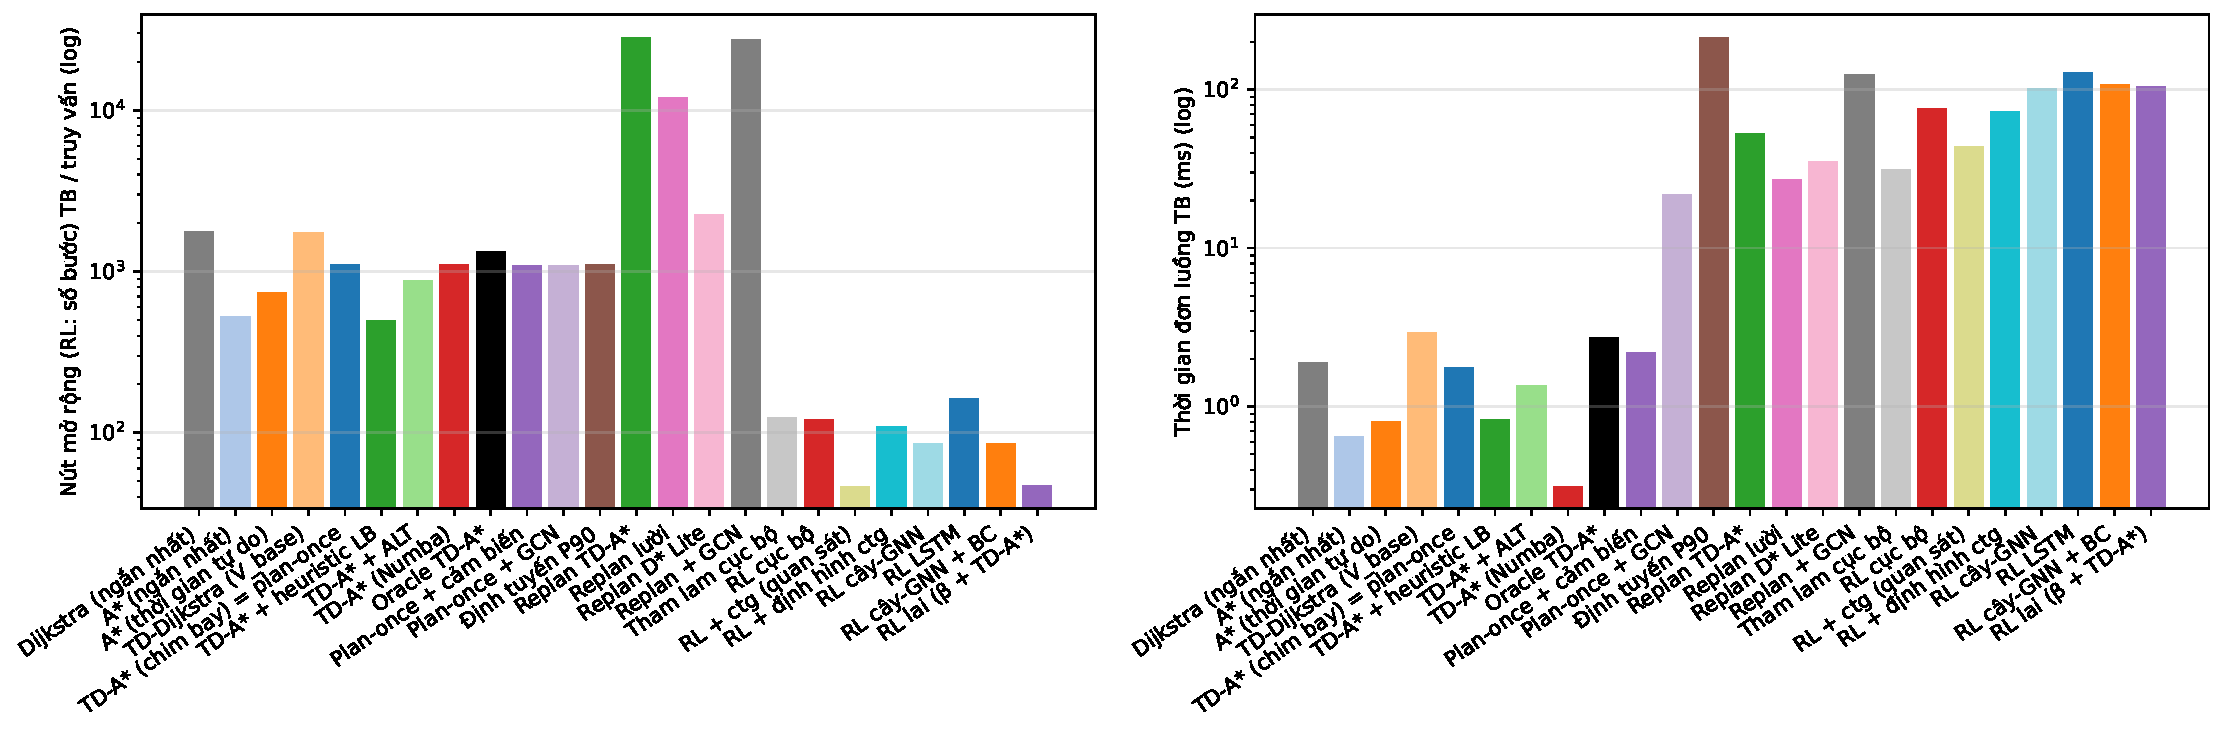
\includegraphics[width=\linewidth]{expansions_runtime.pdf}
\caption{Số nút mở rộng (trái) và thời gian tính đơn luồng (phải) trung bình mỗi truy vấn, thang logarit.}
\label{fig:exp}
\end{figure}

\subsubsection{Vai trò của sự cố và tập stress}

Theo số sự cố trên tập chính (Bảng~\ref{tab:tab_by_incidents}): khi không có sự cố, regret của plan-once chỉ \PoRegretZeroInc\%
và của replan \RpRegretZeroInc\%; với \MaxInc{} sự cố, các con số tương ứng là \PoRegretMaxInc\% và \RpRegretMaxInc\%. Trên tập
stress (Bảng~\ref{tab:tab_stress}), khi sự cố được đặt ưu tiên trên tuyến dự kiến, regret của plan-once tăng lên
\SPoRegret\% trong khi replan giữ \SRpRegret\% và replan + GCN \SRpGnnRegret\%; Dijkstra ngắn nhất \SDijRegret\%. Kết quả xác
nhận giả thuyết H2: tái lập kế hoạch có giá trị chủ yếu khi dự báo sai \emph{cục bộ và lớn}. Bảng~\ref{tab:tab_results_noinc}
cho thấy trên tập con không có sự cố, plan-once đã rất gần oracle, nên lợi ích của TD-A* so với Dijkstra là thật chứ không
do cách đặt sự cố.

\begin{table}[!htbp]
\centering
\small
\caption{Regret trung bình (\%) so với oracle theo số sự cố (chuyến tới đích).}
\label{tab:tab_by_incidents}
\begin{adjustbox}{max width=\linewidth}
\begin{tabular}{lrrrrrrrr}
\toprule
Nhóm & n & Dijkstra (ngắn nhất) & Plan-once TD-A* & Plan-once + GCN & Replan TD-A* & Replan + GCN & RL lai (β + TD-A*) & RL cây-GNN + BC \\
\midrule
0 & 81 & 10{,}48 & 0{,}83 & 0{,}37 & 0{,}35 & 0{,}17 & 0{,}44 & 38{,}50 \\
1 & 57 & 10{,}30 & 1{,}25 & 0{,}44 & 0{,}39 & 0{,}27 & 0{,}55 & 35{,}67 \\
2 & 38 & 12{,}04 & 1{,}16 & 1{,}10 & 0{,}53 & 0{,}25 & 0{,}53 & 35{,}52 \\
3 & 24 & 13{,}05 & 3{,}10 & 0{,}84 & 1{,}00 & 0{,}02 & 1{,}02 & 41{,}69 \\
\bottomrule
\end{tabular}
\end{adjustbox}
\end{table}

\begin{table}[!htbp]
\centering
\small
\caption{Kết quả trên tập stress (sự cố được ưu tiên đặt trên tuyến dự kiến với xác suất 0.7): cùng 200 truy vấn, cùng thời điểm/mức độ sự cố.}
\label{tab:tab_stress}
\begin{adjustbox}{max width=\linewidth}
\begin{tabular}{lrrrrrrrr}
\toprule
Phương pháp & Tới đích (\%) & TB (phút) & Trung vị & P90 & Regret TB (\%) & Regret TV (\%) & Regret P90 (\%) & Dài (km) \\
\midrule
Dijkstra (ngắn nhất) & 100{,}00 & 19{,}38 & 16{,}45 & 33{,}60 & 11{,}38 & 8{,}39 & 26{,}36 & 6{,}26 \\
A* (thời gian tự do) & 100{,}00 & 18{,}80 & 15{,}79 & 33{,}10 & 6{,}38 & 1{,}50 & 19{,}05 & 6{,}64 \\
Plan-once TD-A* & 100{,}00 & 18{,}10 & 15{,}47 & 31{,}84 & 3{,}37 & 0{,}23 & 11{,}44 & 6{,}62 \\
Plan-once + GCN & 100{,}00 & 17{,}88 & 15{,}46 & 31{,}84 & 2{,}10 & 0{,}00 & 5{,}99 & 6{,}58 \\
Định tuyến P90 & 100{,}00 & 18{,}11 & 15{,}56 & 31{,}85 & 3{,}51 & 0{,}52 & 11{,}73 & 6{,}63 \\
Replan TD-A* & 100{,}00 & 17{,}71 & 15{,}28 & 31{,}84 & 0{,}67 & 0{,}00 & 1{,}93 & 6{,}67 \\
Replan lười & 100{,}00 & 17{,}71 & 15{,}28 & 31{,}84 & 0{,}67 & 0{,}00 & 1{,}93 & 6{,}67 \\
Replan D* Lite & 100{,}00 & 17{,}72 & 15{,}28 & 31{,}84 & 0{,}66 & 0{,}00 & 2{,}20 & 6{,}65 \\
Replan + GCN & 100{,}00 & 17{,}64 & 15{,}14 & 31{,}84 & 0{,}31 & 0{,}00 & 0{,}28 & 6{,}64 \\
RL lai (β + TD-A*) & 100{,}00 & 17{,}73 & 15{,}28 & 31{,}84 & 0{,}80 & 0{,}00 & 2{,}33 & 6{,}66 \\
RL cây-GNN + BC & 77{,}50 & 21{,}91 & 18{,}53 & 38{,}82 & 40{,}77 & 26{,}96 & 75{,}24 & 7{,}64 \\
Oracle TD-A* & 100{,}00 & 17{,}57 & 15{,}02 & 31{,}71 & 0{,}00 & 0{,}00 & 0{,}00 & 6{,}66 \\
\bottomrule
\end{tabular}
\end{adjustbox}
\end{table}

\begin{table}[!htbp]
\centering
\small
\caption{Kết quả trên tập con kiểm tra không có sự cố (81 truy vấn).}
\label{tab:tab_results_noinc}
\begin{adjustbox}{max width=\linewidth}
\begin{tabular}{lrrrrrrrr}
\toprule
Phương pháp & Tới đích (\%) & TB (phút) & Trung vị & P90 & Regret TB (\%) & Regret TV (\%) & Regret P90 (\%) & Dài (km) \\
\midrule
Dijkstra (ngắn nhất) & 100{,}00 & 20{,}24 & 15{,}96 & 40{,}92 & 10{,}48 & 7{,}45 & 26{,}73 & 6{,}20 \\
A* (thời gian tự do) & 100{,}00 & 19{,}61 & 14{,}92 & 44{,}10 & 4{,}17 & 0{,}32 & 13{,}68 & 6{,}57 \\
Plan-once TD-A* & 100{,}00 & 18{,}66 & 14{,}77 & 38{,}74 & 0{,}83 & 0{,}00 & 2{,}62 & 6{,}57 \\
Plan-once + GCN & 100{,}00 & 18{,}57 & 14{,}39 & 37{,}68 & 0{,}37 & 0{,}00 & 0{,}97 & 6{,}49 \\
Replan TD-A* & 100{,}00 & 18{,}56 & 14{,}43 & 38{,}49 & 0{,}35 & 0{,}00 & 1{,}58 & 6{,}58 \\
Replan + GCN & 100{,}00 & 18{,}51 & 14{,}39 & 37{,}62 & 0{,}17 & 0{,}00 & 0{,}00 & 6{,}55 \\
RL lai (β + TD-A*) & 100{,}00 & 18{,}57 & 14{,}43 & 38{,}49 & 0{,}44 & 0{,}00 & 1{,}66 & 6{,}58 \\
Oracle TD-A* & 100{,}00 & 18{,}47 & 14{,}39 & 37{,}62 & 0{,}00 & 0{,}00 & 0{,}00 & 6{,}59 \\
\bottomrule
\end{tabular}
\end{adjustbox}
\end{table}


\subsubsection{Mức nhiễu, dự báo GCN và định tuyến P90}

GCN giảm RMSE \eqref{eq:rmse} của log-tỉ số vận tốc trên các cạnh chưa quan sát từ \GcnRmseZero{} (dự báo nền) xuống
\GcnRmse{}, tức giảm \GcnImprove\% (Bảng~\ref{tab:tab_forecast}, Hình~\ref{fig:gcn}). Lợi ích này chuyển thành chất lượng tuyến
và tăng theo mức nhiễu (Hình~\ref{fig:noise}, Bảng~\ref{tab:tab_noise_sweep}): với $\sigma=\NoiseMaxSigma$ và không có sự cố,
regret của plan-once là \NoisePoMax\%, plan-once + GCN \NoisePoGnnMax\%, replan \NoiseRpMax\%, replan + GCN \NoiseRpGnnMax\% và
Dijkstra \NoiseDijMax\%. Điều này chỉ xảy ra vì nhiễu có tương quan không gian--thời gian; với nhiễu độc lập (phiên bản đầu
của dự án) quan sát không mang thông tin về các cạnh khác nên không có gì để lan truyền.

\begin{table}[!htbp]
\centering
\small
\caption{Sai số dự báo log-tỉ số vận tốc (mốc $h$ và $h+1$) trên 20 trường kiểm định độc lập; 1341 cảm biến (15\% cạnh) + cạnh trong bán kính quan sát.}
\label{tab:tab_forecast}
\begin{adjustbox}{max width=\linewidth}
\begin{tabular}{lrr}
\toprule
Mô hình & RMSE cạnh chưa quan sát & RMSE mọi cạnh \\
\midrule
Dự báo nền V\_base (log-tỉ số = 0) & 0{,}1959 & 0{,}1965 \\
GCN chưa huấn luyện & 0{,}2375 & 0{,}2381 \\
GCN đã huấn luyện & 0{,}1602 & 0{,}1526 \\
\bottomrule
\end{tabular}
\end{adjustbox}
\end{table}


\begin{figure}[H]
\centering
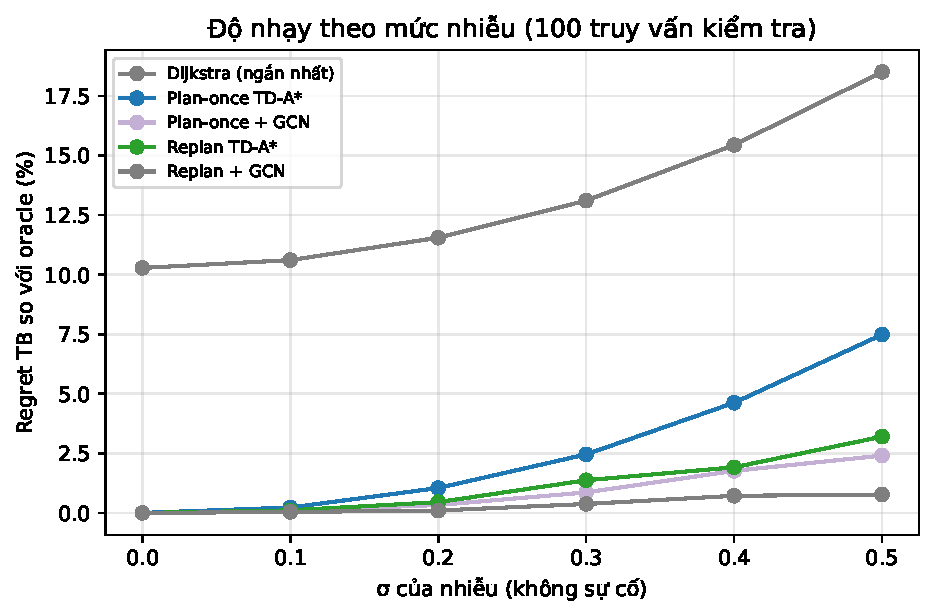
\includegraphics[width=0.49\linewidth]{noise_sensitivity.pdf}\hfill
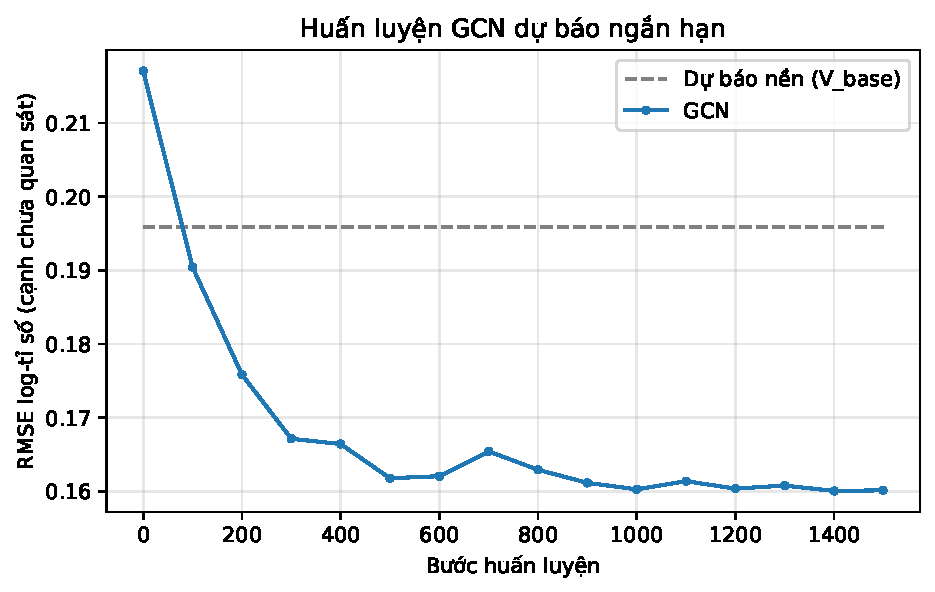
\includegraphics[width=0.49\linewidth]{gcn_training.pdf}
\caption{Trái: regret theo mức nhiễu $\sigma$ khi không có sự cố. Phải: RMSE trên cạnh chưa quan sát trong quá trình huấn
luyện GCN.}
\label{fig:noise}\label{fig:gcn}
\end{figure}

\begin{table}[!htbp]
\centering
\small
\caption{Regret trung bình (\%) theo mức nhiễu $\sigma$ khi không có sự cố.}
\label{tab:tab_noise_sweep}
\begin{adjustbox}{max width=\linewidth}
\begin{tabular}{lrrrrr}
\toprule
$\sigma$ & Dijkstra (ngắn nhất) & Plan-once TD-A* & Plan-once + GCN & Replan TD-A* & Replan + GCN \\
\midrule
0{,}00 & 10{,}28 & 0{,}00 & 0{,}00 & 0{,}00 & 0{,}00 \\
0{,}10 & 10{,}61 & 0{,}23 & 0{,}09 & 0{,}11 & 0{,}04 \\
0{,}20 & 11{,}55 & 1{,}05 & 0{,}33 & 0{,}45 & 0{,}10 \\
0{,}30 & 13{,}11 & 2{,}46 & 0{,}86 & 1{,}37 & 0{,}38 \\
0{,}40 & 15{,}44 & 4{,}62 & 1{,}77 & 1{,}92 & 0{,}72 \\
0{,}50 & 18{,}51 & 7{,}49 & 2{,}41 & 3{,}20 & 0{,}77 \\
\bottomrule
\end{tabular}
\end{adjustbox}
\end{table}


\textbf{Định tuyến P90 không mang lại lợi ích.} Trên \RiskEvalNQ{} truy vấn, mỗi tuyến được đánh giá trên 100 kịch bản độc
lập (Bảng~\ref{tab:tab_risk}). Tuyến P90 khác tuyến plan-once ở \RiskChangedPct\% số truy vấn, nhưng ở các truy vấn đó phân vị
90\% thực tế thay đổi trung bình \RiskDiffPnChanged{} phút (dương nghĩa là tệ hơn) và chỉ tốt hơn ở \RiskBetterPnPct\% số truy
vấn. Có hai nguyên nhân: (i) với $M=\RiskM$ kịch bản, phân vị ước lượng có sai số đáng kể, nên việc chọn ứng viên có phân vị
\emph{ước lượng} nhỏ nhất dẫn đến hiện tượng ``lời nguyền người thắng'' --- ứng viên được chọn thường là ứng viên được ước
lượng thấp hơn thực tế; (ii) trong mô phỏng, các tuyến ứng viên chồng lấp nhiều và nhiễu tương quan không gian khiến chúng
chịu rủi ro gần như nhau, nên không tồn tại tuyến ``an toàn'' rõ rệt.

\begin{table}[!htbp]
\centering
\small
\caption{Độ tin cậy tuyến trên 100 kịch bản nhiễu độc lập cho mỗi truy vấn (100 truy vấn kiểm tra, không sự cố). Tuyến P90 khác tuyến plan-once ở 20\% truy vấn.}
\label{tab:tab_risk}
\begin{adjustbox}{max width=\linewidth}
\begin{tabular}{lrrr}
\toprule
Tuyến & TB thời gian (phút) & P90 (phút) & Độ lệch chuẩn \\
\midrule
Plan-once TD-A* & 16{,}787 & 17{,}691 & 0{,}709 \\
Định tuyến P90 & 16{,}798 & 17{,}708 & 0{,}710 \\
\bottomrule
\end{tabular}
\end{adjustbox}
\end{table}


\subsubsection{Theo giờ xuất phát và khoảng cách}

Regret của tuyến ngắn nhất \emph{thấp hơn} vào giờ cao điểm (\DijRegretPeak\%) so với thấp điểm (\DijRegretOff\%)
(Bảng~\ref{tab:tab_by_peak}, Hình~\ref{fig:hour}). Phân tích tuyến nhanh nhất so với tuyến ngắn nhất trên vận tốc nền
(Hình~\ref{fig:saving}, Bảng~\ref{tab:tab_saving_by_hour}) xác nhận: tuyến nhanh nhất tiết kiệm \SavingThree\% lúc 3h nhưng chỉ
\SavingEight\% lúc 8h và \SavingEighteen\% lúc 18h. Nguyên nhân nằm ở mô hình: trục chính có độ nhạy và hệ số trục nóng cao
nhất nên vào cao điểm chậm gần bằng đường nhánh (Hình~\ref{fig:speedcurves}); lợi thế ``đi đường lớn dù xa hơn'' biến mất và
tuyến nhanh nhất hội tụ về tuyến ngắn. Đây là hệ quả của giả định mô phỏng và cần được kiểm chứng với dữ liệu thật; về
tuyệt đối, chuyến đi vẫn dài hơn nhiều vào cao điểm (tuyến ngắn nhất \TTShortEight{} phút lúc 8h so với \TTShortThree{} phút
lúc 3h). Theo khoảng cách (Bảng~\ref{tab:tab_by_distance}), regret tương đối của plan-once giảm khi chuyến đi dài hơn vì một
sự cố chiếm tỉ trọng nhỏ hơn trong tổng thời gian.

\begin{figure}[H]
\centering
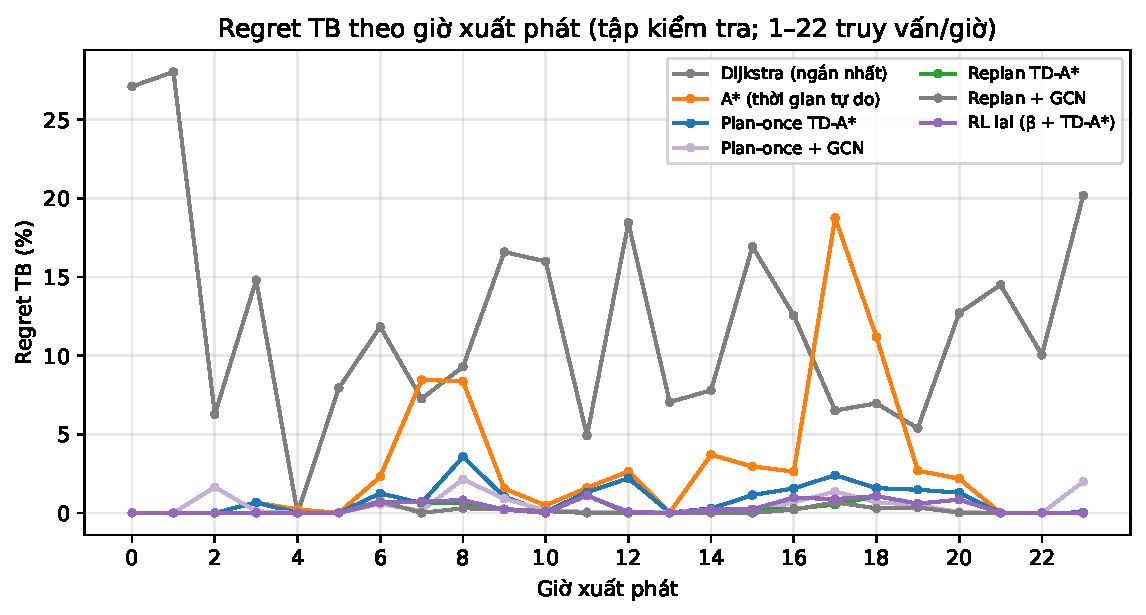
\includegraphics[width=0.49\linewidth]{regret_by_hour.pdf}\hfill
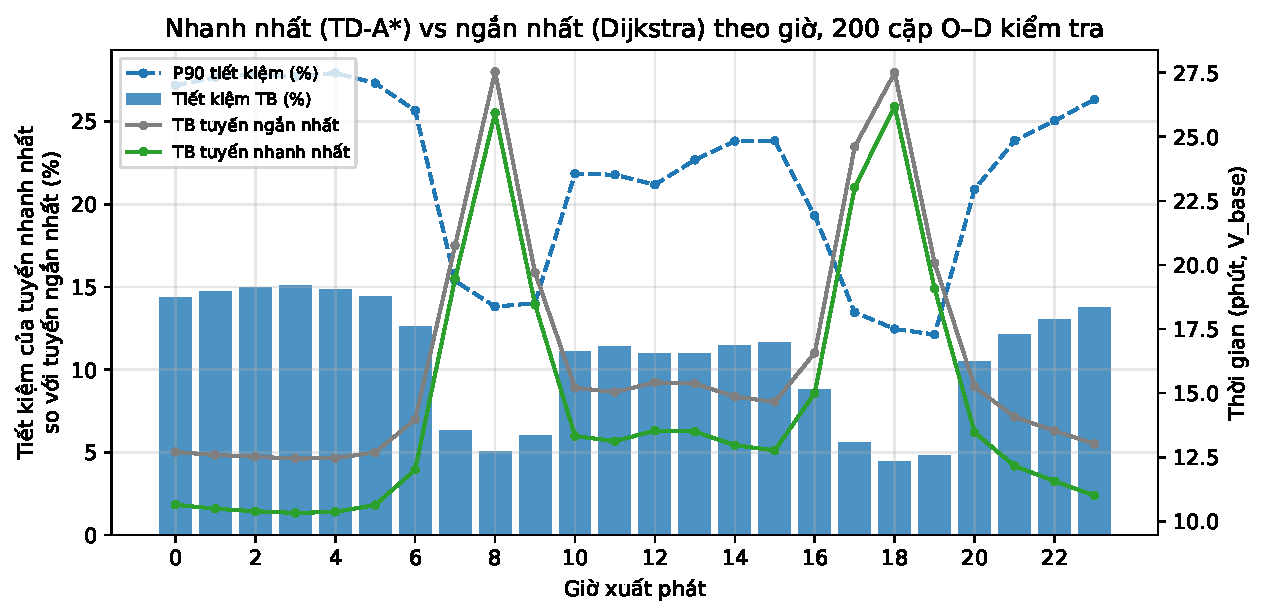
\includegraphics[width=0.49\linewidth]{saving_by_hour.pdf}
\caption{Trái: regret theo giờ xuất phát. Phải: tiết kiệm của tuyến nhanh nhất so với tuyến ngắn nhất theo giờ.}
\label{fig:hour}\label{fig:saving}
\end{figure}

\begin{table}[!htbp]
\centering
\small
\caption{Regret trung bình (\%) so với oracle theo giờ xuất phát (cao điểm: 7h, 8h, 17h, 18h) (chuyến tới đích).}
\label{tab:tab_by_peak}
\begin{adjustbox}{max width=\linewidth}
\begin{tabular}{lrrrrrrrr}
\toprule
Nhóm & n & Dijkstra (ngắn nhất) & Plan-once TD-A* & Plan-once + GCN & Replan TD-A* & Replan + GCN & RL lai (β + TD-A*) & RL cây-GNN + BC \\
\midrule
cao điểm & 74 & 7{,}46 & 1{,}91 & 0{,}98 & 0{,}76 & 0{,}29 & 0{,}88 & 28{,}20 \\
thấp điểm & 126 & 13{,}13 & 0{,}92 & 0{,}36 & 0{,}31 & 0{,}14 & 0{,}37 & 42{,}46 \\
\bottomrule
\end{tabular}
\end{adjustbox}
\end{table}

\begin{table}[!htbp]
\centering
\small
\caption{Regret trung bình (\%) so với oracle theo khoảng cách O–D (chuyến tới đích).}
\label{tab:tab_by_distance}
\begin{adjustbox}{max width=\linewidth}
\begin{tabular}{lrrrrrrrr}
\toprule
Nhóm & n & Dijkstra (ngắn nhất) & Plan-once TD-A* & Plan-once + GCN & Replan TD-A* & Replan + GCN & RL lai (β + TD-A*) & RL cây-GNN + BC \\
\midrule
ngan (<2.5km) & 42 & 10{,}18 & 1{,}39 & 0{,}34 & 0{,}31 & 0{,}11 & 0{,}48 & 37{,}09 \\
trung binh (2.5-4.5km) & 67 & 10{,}86 & 1{,}32 & 0{,}88 & 0{,}60 & 0{,}32 & 0{,}66 & 35{,}11 \\
xa (>4.5km) & 91 & 11{,}56 & 1{,}21 & 0{,}48 & 0{,}45 & 0{,}14 & 0{,}51 & 39{,}63 \\
\bottomrule
\end{tabular}
\end{adjustbox}
\end{table}

\begin{table}[!htbp]
\centering
\small
\caption{Regret trung bình (\%) so với oracle theo mức nhiễu $\sigma$ (chuyến tới đích).}
\label{tab:tab_by_sigma}
\begin{adjustbox}{max width=\linewidth}
\begin{tabular}{lrrrrrrrr}
\toprule
Nhóm & n & Dijkstra (ngắn nhất) & Plan-once TD-A* & Plan-once + GCN & Replan TD-A* & Replan + GCN & RL lai (β + TD-A*) & RL cây-GNN + BC \\
\midrule
0.05 & 76 & 10{,}84 & 0{,}46 & 0{,}54 & 0{,}04 & 0{,}04 & 0{,}04 & 36{,}15 \\
0.15 & 56 & 8{,}49 & 0{,}61 & 0{,}30 & 0{,}25 & 0{,}13 & 0{,}26 & 39{,}16 \\
0.3 & 68 & 13{,}34 & 2{,}77 & 0{,}88 & 1{,}14 & 0{,}41 & 1{,}38 & 37{,}38 \\
\bottomrule
\end{tabular}
\end{adjustbox}
\end{table}

\begin{table}[!htbp]
\centering
\small
\caption{Tiết kiệm thời gian của tuyến nhanh nhất so với tuyến ngắn nhất (trên vận tốc nền) theo giờ xuất phát.}
\label{tab:tab_saving_by_hour}
\begin{adjustbox}{max width=\linewidth}
\begin{tabular}{lrrrrr}
\toprule
Giờ & Ngắn nhất (phút) & Nhanh nhất (phút) & Tiết kiệm TB (\%) & P90 (\%) & Dài thêm (\%) \\
\midrule
0 & 12{,}70 & 10{,}64 & 14{,}38 & 27{,}19 & 6{,}1 \\
3 & 12{,}45 & 10{,}33 & 15{,}06 & 27{,}72 & 6{,}1 \\
6 & 13{,}96 & 12{,}01 & 12{,}61 & 25{,}67 & 5{,}4 \\
7 & 20{,}76 & 19{,}47 & 6{,}30 & 15{,}37 & 3{,}7 \\
8 & 27{,}53 & 25{,}93 & 5{,}06 & 13{,}81 & 3{,}9 \\
9 & 19{,}70 & 18{,}46 & 6{,}01 & 14{,}02 & 4{,}2 \\
12 & 15{,}42 & 13{,}54 & 10{,}96 & 21{,}18 & 4{,}9 \\
14 & 14{,}86 & 12{,}97 & 11{,}44 & 23{,}82 & 5{,}0 \\
16 & 16{,}57 & 15{,}00 & 8{,}81 & 19{,}31 & 4{,}1 \\
17 & 24{,}61 & 23{,}03 & 5{,}61 & 13{,}47 & 5{,}9 \\
18 & 27{,}50 & 26{,}18 & 4{,}45 & 12{,}46 & 6{,}0 \\
19 & 20{,}07 & 19{,}07 & 4{,}81 & 12{,}12 & 3{,}3 \\
21 & 14{,}07 & 12{,}16 & 12{,}15 & 23{,}83 & 5{,}3 \\
\bottomrule
\end{tabular}
\end{adjustbox}
\end{table}


\begin{figure}[H]
\centering
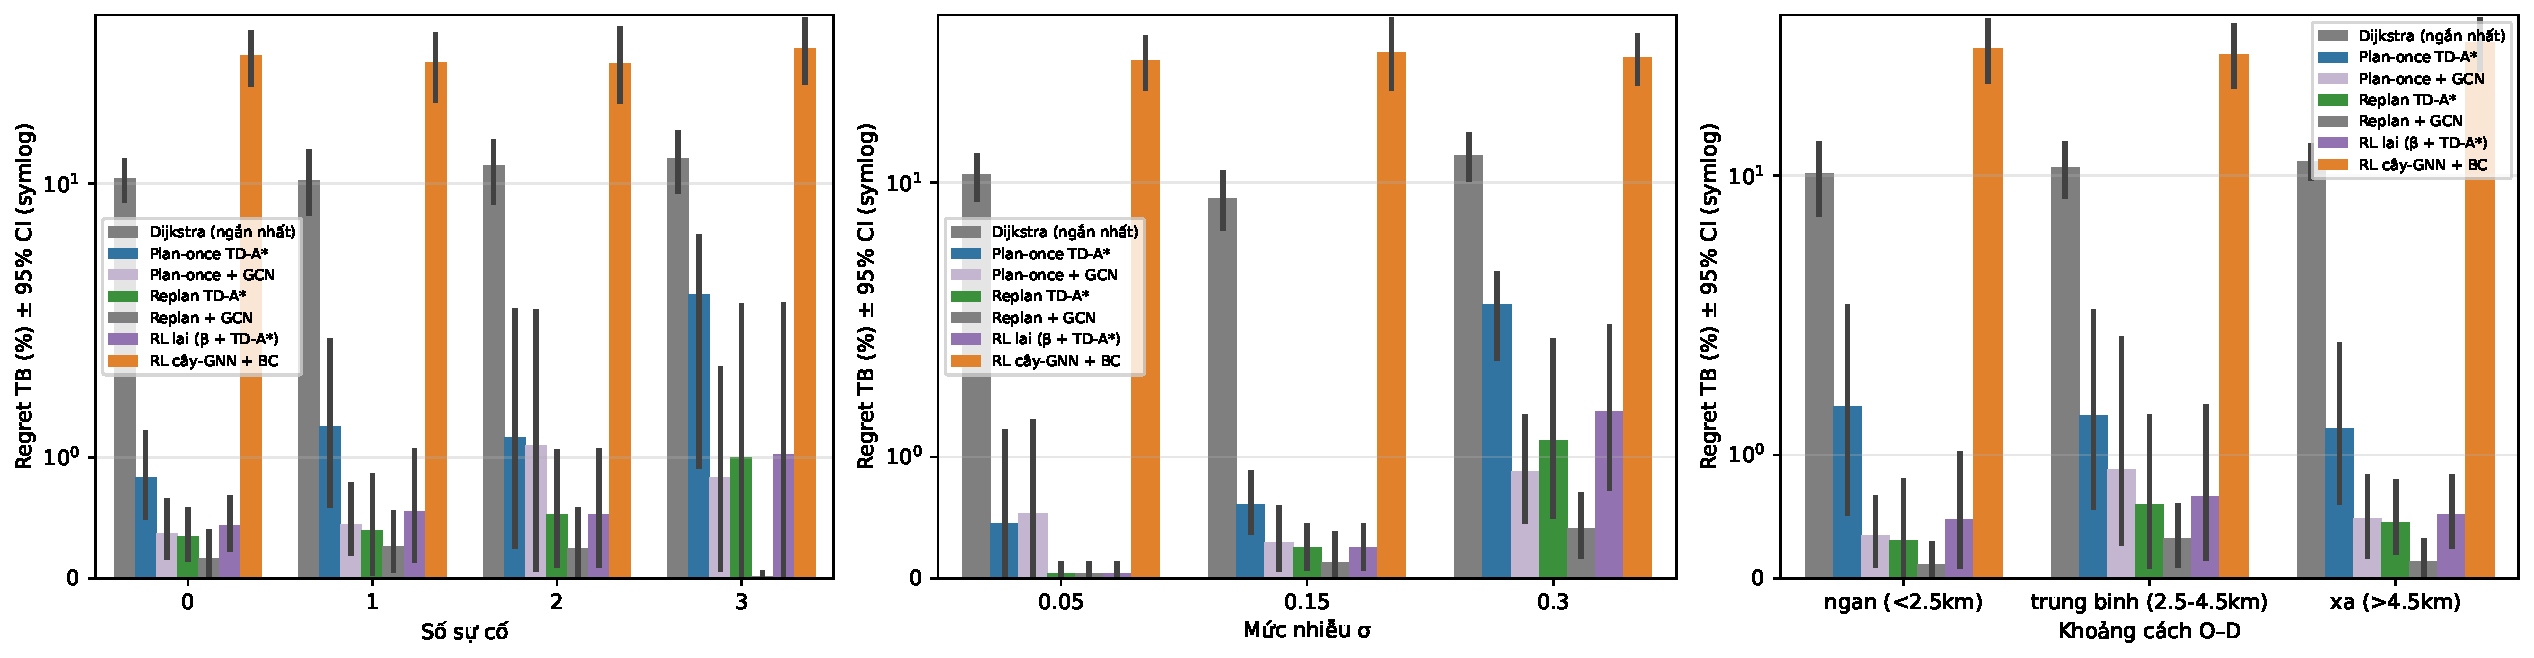
\includegraphics[width=\linewidth]{regret_breakdowns.pdf}
\caption{Regret theo số sự cố, mức nhiễu và khoảng cách (thanh lỗi: khoảng tin cậy bootstrap 95\%; trục symlog).}
\label{fig:breakdown}
\end{figure}

\subsubsection{Học tăng cường}

Bảng~\ref{tab:tab_main_rl} (seed tốt nhất theo tập kiểm định), Bảng~\ref{tab:tab_rl_seeds} (mọi seed) và Hình~\ref{fig:rl}
trình bày kết quả RL. Tỉ lệ tới đích trên tập kiểm tra, trung bình qua 3 seed: RL cục bộ \RlSeedSucc\%, RL + định hình ctg
\RlShapeSeedSucc\%, RL cây-GNN \RlTreeSeedSucc\%, RL cây-GNN + BC \RlTreeBcSeedSucc\%, RL LSTM \RlLstmSeedSucc\%; baseline tham
lam thủ công đạt \GrSuccess\%.

\begin{table}[!htbp]
\centering
\small
\caption{Kết quả các biến thể học tăng cường (seed tốt nhất theo tập kiểm định) và baseline tham lam trên cùng tập kiểm tra; thời gian và regret chỉ tính trên các chuyến tới đích.}
\label{tab:tab_main_rl}
\begin{adjustbox}{max width=\linewidth}
\begin{tabular}{lrrrrrrrr}
\toprule
Phương pháp & Tới đích (\%) & TB (phút) & Trung vị & P90 & Regret TB (\%) & Regret TV (\%) & Regret P90 (\%) & Dài (km) \\
\midrule
Tham lam cục bộ & 37{,}50 & 21{,}02 & 17{,}56 & 38{,}70 & 62{,}88 & 43{,}80 & 135{,}28 & 6{,}75 \\
RL cục bộ & 35{,}00 & 22{,}27 & 18{,}83 & 42{,}88 & 63{,}24 & 35{,}74 & 90{,}16 & 7{,}17 \\
RL + ctg (quan sát) & 100{,}00 & 18{,}32 & 15{,}23 & 31{,}52 & 5{,}19 & 0{,}82 & 17{,}79 & 6{,}64 \\
RL + định hình ctg & 57{,}00 & 24{,}18 & 20{,}50 & 43{,}68 & 76{,}11 & 49{,}93 & 183{,}88 & 7{,}87 \\
RL cây-GNN & 67{,}00 & 20{,}55 & 18{,}60 & 35{,}43 & 39{,}38 & 35{,}44 & 87{,}93 & 7{,}31 \\
RL LSTM & 2{,}50 & 22{,}83 & 23{,}23 & 29{,}17 & 219{,}06 & 230{,}42 & 307{,}75 & 6{,}36 \\
RL cây-GNN + BC & 77{,}00 & 21{,}59 & 17{,}74 & 40{,}35 & 37{,}36 & 23{,}74 & 73{,}33 & 7{,}57 \\
RL lai (β + TD-A*) & 100{,}00 & 17{,}37 & 14{,}47 & 30{,}89 & 0{,}56 & 0{,}00 & 1{,}67 & 6{,}63 \\
Replan TD-A* & 100{,}00 & 17{,}35 & 14{,}47 & 30{,}89 & 0{,}47 & 0{,}00 & 1{,}18 & 6{,}63 \\
Oracle TD-A* & 100{,}00 & 17{,}26 & 14{,}47 & 30{,}89 & 0{,}00 & 0{,}00 & 0{,}00 & 6{,}64 \\
\bottomrule
\end{tabular}
\end{adjustbox}
\end{table}


\begin{figure}[H]
\centering
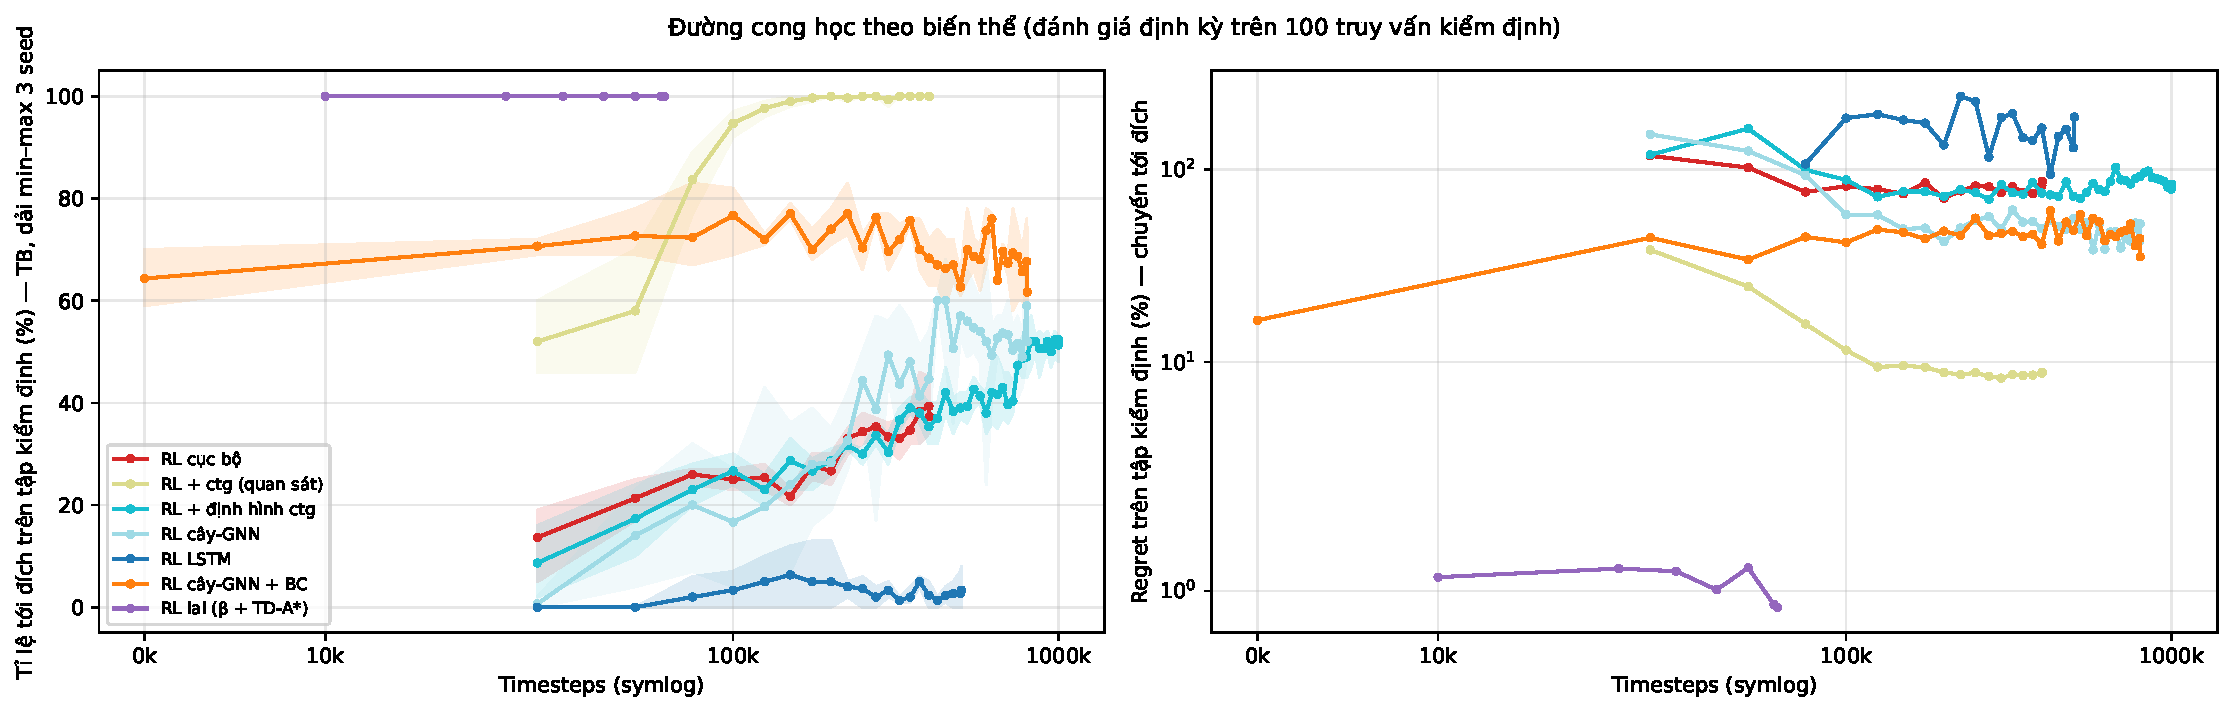
\includegraphics[width=\linewidth]{rl_learning_curves.pdf}
\caption{Đường cong học trên tập kiểm định: trung bình và dải min--max qua 3 seed (trục hoành symlog).}
\label{fig:rl}
\end{figure}

\textbf{Cải tiến nào có tác dụng?}
\begin{itemize}
    \item \emph{Quan sát rộng hơn có tác dụng lớn nhất trong nhóm chọn từng cạnh.} Cây lân cận \TreeDepth{} bước với GNN nâng
    tỉ lệ tới đích từ \RlSuccess\% lên \RlTreeSuccess\% và giảm regret từ \RlRegret\% xuống \RlTreeRegret\%: tác tử nhìn thấy ngõ
    cụt phía trước (\DeadEndPct\% số nút là ngõ cụt) thay vì chỉ thấy hướng chim bay. Đường cong học vẫn đang đi lên ở cuối ngân
    sách, nên huấn luyện lâu hơn có thể còn cải thiện.
    \item \emph{Học bắt chước cho kết quả tốt nhất.} Chỉ riêng giai đoạn BC đã đạt độ chính xác bắt chước \RlTreeBcBcAcc\% và
    \RlTreeBcAfterBc\% tới đích trên tập kiểm định (trung bình 3 seed) trước khi chạy PPO; seed được chọn đạt \RlTreeBcSuccess\%
    trên tập kiểm tra (regret \RlTreeBcRegret\%). Tuy nhiên PPO tinh chỉnh \emph{không} cải thiện thêm mà làm chính sách dao động
    và giảm dần (Hình~\ref{fig:rl}); checkpoint tốt nhất thường xuất hiện sớm. Đây là hiện tượng thường gặp khi tinh chỉnh bằng
    gradient chính sách với phần thưởng thưa sau giai đoạn bắt chước.
    \item \emph{Định hình theo cost-to-go} tăng tỉ lệ tới đích (\RlShapeSuccess\% so với \RlSuccess\%) nhưng regret trên các
    chuyến tới đích không giảm (\RlShapeRegret\%): định hình chỉ hướng tác tử về đích mà không dạy nó tránh đoạn chậm.
    \item \emph{Bộ nhớ LSTM thất bại} (\RlLstmSuccess\%): RecurrentPPO không có mặt nạ hành động nên phải ánh xạ $a\bmod\deg^+(u)$,
    làm ý nghĩa của mỗi đầu ra thay đổi theo bậc của nút; cộng với tốc độ học chậm hơn nhiều, chính sách không thoát khỏi việc
    đi lòng vòng.
    \item \emph{Thí nghiệm đối chứng có thông tin toàn cục} (cost-to-go trong quan sát) tới đích \RlcSuccess\% với regret
    \RlcRegret\%, nhưng tuyến của nó trùng hệt tuyến A* thời gian tự do ở \RouteSameRlcFf\% số truy vấn và thời gian không khác
    biệt so với A* tự do (Bảng~\ref{tab:tab_stat_tests}): chính sách chủ yếu bám theo gradient của cost-to-go tĩnh.
    \item \emph{RL lai đạt 100\% tới đích với regret \RlHybRegret\%} nhưng không vượt được replan thuần (\RpRegret\%): hiệu
    \DiffRlHybridReplan{} phút mỗi chuyến, khoảng tin cậy \CiRlHybridReplan, Wilcoxon $p$ \PRlHybridReplan. Tác tử học được
    $\bar\beta=\HybMeanBeta$, gần với $\beta=1$ của replan, và tuyến trùng replan ở \RouteSameRlHybRp\% số truy vấn. Giá trị của RL
    ở đây là \emph{giữ được} bảo đảm tới đích và chất lượng của tìm kiếm, chứ chưa tạo thêm lợi ích.
\end{itemize}
Mọi biến thể RL chọn từng cạnh vẫn kém plan-once rất xa: biến thể tốt nhất (cây-GNN + BC) chậm hơn plan-once
\DiffRlTreeBcPlanOnce{} phút mỗi chuyến trên các truy vấn nó tới đích (\CiRlTreeBcPlanOnce) và chỉ tốt hơn ở
\BetterRlTreeBcPlanOnce\% số truy vấn. Kết quả xác nhận giả thuyết H3.

\begin{table}[!htbp]
\centering
\small
\caption{Kết quả học tăng cường theo từng seed (checkpoint tốt nhất theo tập kiểm định; cột Chọn đánh dấu seed dùng cho bảng chính).}
\label{tab:tab_rl_seeds}
\begin{adjustbox}{max width=\linewidth}
\begin{tabular}{lrrrrrrrc}
\toprule
Biến thể & Seed & Bước & Val tới đích (\%) & Tốt nhất tại & Test tới đích (\%) & Test regret (\%) & Huấn luyện (phút) & Chọn \\
\midrule
RL cục bộ & 0 & 401408 & 46{,}0 & 375000 & 35{,}0 & 63{,}24 & 21{,}5 & x \\
RL cục bộ & 1 & 401408 & 39{,}0 & 400000 & 37{,}0 & 62{,}18 & 19{,}4 &  \\
RL cục bộ & 2 & 401408 & 37{,}0 & 375000 & 38{,}0 & 66{,}14 & 19{,}8 &  \\
RL + ctg (quan sát) & 0 & 401408 & 100{,}0 & 275000 & 99{,}0 & 5{,}34 & 21{,}1 &  \\
RL + ctg (quan sát) & 1 & 401408 & 100{,}0 & 400000 & 100{,}0 & 5{,}19 & 21{,}1 & x \\
RL + ctg (quan sát) & 2 & 401408 & 100{,}0 & 300000 & 99{,}5 & 5{,}16 & 14{,}9 &  \\
RL + định hình ctg & 0 & 1003520 & 57{,}0 & 825000 & 57{,}0 & 76{,}11 & 50{,}7 & x \\
RL + định hình ctg & 1 & 1003520 & 52{,}0 & 925000 & 49{,}5 & 63{,}25 & 50{,}6 &  \\
RL + định hình ctg & 2 & 1003520 & 53{,}0 & 1000000 & 58{,}5 & 72{,}94 & 51{,}4 &  \\
RL cây-GNN & 0 & 802816 & 68{,}0 & 600000 & 67{,}0 & 39{,}38 & 153{,}9 & x \\
RL cây-GNN & 1 & 802816 & 65{,}0 & 475000 & 74{,}0 & 54{,}33 & 153{,}5 &  \\
RL cây-GNN & 2 & 802816 & 60{,}0 & 800000 & 63{,}0 & 42{,}31 & 155{,}5 &  \\
RL LSTM & 0 & 503808 & 1{,}0 & 450000 & 2{,}5 & 219{,}06 & 169{,}7 & x \\
RL LSTM & 1 & 503808 & 13{,}0 & 175000 & 8{,}5 & 175{,}38 & 138{,}6 &  \\
RL LSTM & 2 & 503808 & 2{,}0 & 425000 & 1{,}0 & 280{,}42 & 138{,}5 &  \\
RL cây-GNN + BC & 0 & 802816 & 82{,}0 & 100000 & 77{,}0 & 37{,}36 & 160{,}7 & x \\
RL cây-GNN + BC & 1 & 802816 & 83{,}0 & 225000 & 86{,}0 & 42{,}94 & 160{,}9 &  \\
RL cây-GNN + BC & 2 & 802816 & 77{,}0 & 625000 & 76{,}5 & 45{,}54 & 161{,}2 &  \\
RL lai (β + TD-A*) & 0 & 61440 & 100{,}0 & 30000 & 100{,}0 & 0{,}56 & 11{,}5 & x \\
RL lai (β + TD-A*) & 1 & 61440 & 100{,}0 & 61440 & 100{,}0 & 0{,}90 & 11{,}4 &  \\
RL lai (β + TD-A*) & 2 & 61440 & 100{,}0 & 60000 & 100{,}0 & 0{,}50 & 11{,}2 &  \\
\bottomrule
\end{tabular}
\end{adjustbox}
\end{table}

\begin{table}[!htbp]
\centering
\small
\caption{Độ trùng tuyến giữa các cặp phương pháp trên tập kiểm tra chính.}
\label{tab:tab_route_overlap}
\begin{adjustbox}{max width=\linewidth}
\begin{tabular}{lrrr}
\toprule
Cặp phương pháp & n & Tuyến giống hệt (\%) & Jaccard cạnh TB (\%) \\
\midrule
RL + ctg (quan sát) vs A* (thời gian tự do) & 200 & 64{,}0 & 91{,}7 \\
RL cây-GNN + BC vs Oracle TD-A* & 200 & 3{,}5 & 32{,}1 \\
RL cây-GNN + BC vs Plan-once TD-A* & 200 & 2{,}5 & 31{,}6 \\
RL lai (β + TD-A*) vs Replan TD-A* & 200 & 93{,}5 & 98{,}1 \\
Plan-once TD-A* vs Oracle TD-A* & 200 & 57{,}5 & 84{,}1 \\
Replan TD-A* vs Oracle TD-A* & 200 & 81{,}5 & 91{,}0 \\
Replan lười vs Replan TD-A* & 200 & 96{,}0 & 99{,}1 \\
Replan D* Lite vs Replan TD-A* & 200 & 88{,}0 & 94{,}9 \\
Replan + GCN vs Replan TD-A* & 200 & 86{,}5 & 92{,}2 \\
Định tuyến P90 vs Plan-once TD-A* & 200 & 77{,}5 & 94{,}6 \\
A* (thời gian tự do) vs Dijkstra (ngắn nhất) & 200 & 12{,}5 & 47{,}1 \\
\bottomrule
\end{tabular}
\end{adjustbox}
\end{table}


\begin{figure}[H]
\centering
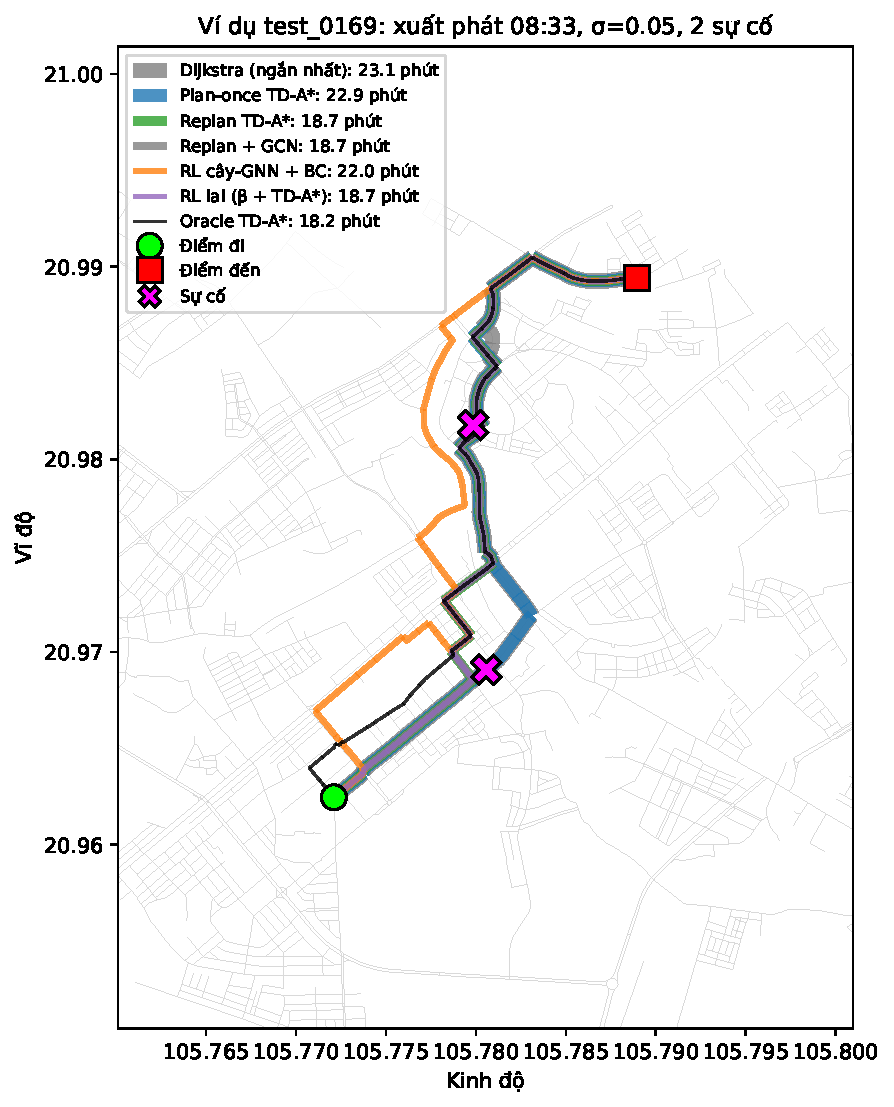
\includegraphics[width=0.66\linewidth]{route_example.pdf}
\caption{Ví dụ truy vấn \ExampleQuery{} (truy vấn có sự cố với chênh lệch giữa plan-once và replan lớn nhất).}
\label{fig:route}
\end{figure}

\subsubsection{Chọn giờ xuất phát}

Bảng~\ref{tab:tab_departure} và Hình~\ref{fig:dep} trình bày kết quả. Khi tính đủ thời gian chờ ($w=1$), chờ không bao giờ
có lợi trên tập kiểm tra (lời giải vét cạn chọn chờ ở \DepOptWOneWait\% số truy vấn) và Q-learning học đúng chính sách ``đi
ngay''. Khi chờ rẻ hơn ($w=\DepLowW$), lời giải vét cạn chọn chờ ở \DepOptWLowWait\% số truy vấn và giảm chi phí trung bình
từ \DepGoWLowCost{} xuống \DepOptWLowCost{} phút --- có truy vấn tiết kiệm tới \DepMaxSaving{} phút nhờ tránh cao điểm --- nhưng
Q-learning dạng bảng \emph{không} nhận diện được các truy vấn đó: chi phí \DepQWLowCost{} phút, regret \DepQWLowRegret{} phút
so với \DepGoWLowRegret{} phút của ``đi ngay''. Trong lần chạy đầu, việc khởi tạo $Q=0$ (lạc quan vì mọi phần thưởng đều âm)
khiến tác tử chờ quá nhiều ở các trạng thái hiếm gặp; quy tắc chỉ tin $Q$ ở ô đã cập nhật đủ \DepMinVisits{} lần
(Mục~\ref{sec:method:departure}) đã khắc phục phần lớn vấn đề này.

\begin{table}[!htbp]
\centering
\small
\caption{Kết quả thí nghiệm chọn giờ xuất phát trên tập kiểm tra (bước chờ 10 phút, tối đa 6 lần).}
\label{tab:tab_departure}
\begin{adjustbox}{max width=\linewidth}
\begin{tabular}{llrrrrr}
\toprule
w & Chính sách & Chi phí TB (phút) & Đi TB (phút) & Chờ+đi TB (phút) & Tỉ lệ chờ & Regret (phút) \\
\midrule
0{,}25 & Đi ngay & 17{,}26 & 17{,}26 & 17{,}26 & 0{,}000 & 0{,}183 \\
0{,}25 & Giờ tối ưu (vét cạn) & 17{,}08 & 16{,}62 & 18{,}47 & 0{,}050 & 0{,}000 \\
0{,}25 & Q-learning & 17{,}73 & 16{,}75 & 20{,}65 & 0{,}160 & 0{,}649 \\
0{,}50 & Đi ngay & 17{,}26 & 17{,}26 & 17{,}26 & 0{,}000 & 0{,}007 \\
0{,}50 & Giờ tối ưu (vét cạn) & 17{,}26 & 17{,}18 & 17{,}33 & 0{,}010 & 0{,}000 \\
0{,}50 & Q-learning & 17{,}55 & 17{,}10 & 18{,}00 & 0{,}060 & 0{,}294 \\
1{,}00 & Đi ngay & 17{,}26 & 17{,}26 & 17{,}26 & 0{,}000 & 0{,}000 \\
1{,}00 & Giờ tối ưu (vét cạn) & 17{,}26 & 17{,}26 & 17{,}26 & 0{,}000 & 0{,}000 \\
1{,}00 & Q-learning & 17{,}26 & 17{,}26 & 17{,}26 & 0{,}000 & 0{,}000 \\
\bottomrule
\end{tabular}
\end{adjustbox}
\end{table}


\begin{figure}[H]
\centering
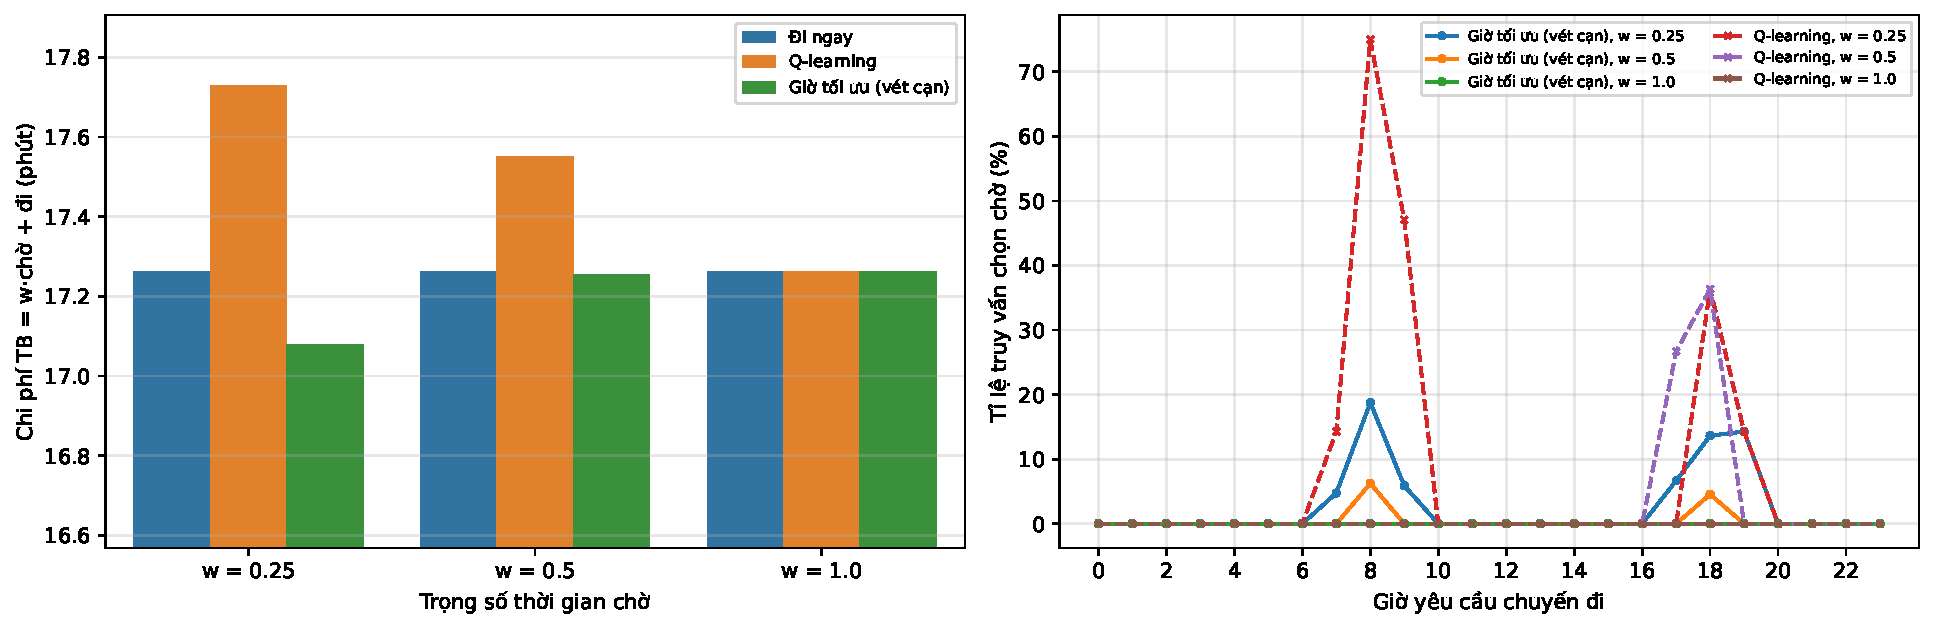
\includegraphics[width=\linewidth]{departure_time.pdf}
\caption{Chọn giờ xuất phát: chi phí trung bình theo chính sách (trái) và tỉ lệ chọn chờ theo giờ (phải).}
\label{fig:dep}
\end{figure}

\subsubsection{Nhiều xe cùng được dẫn đường}

Khi \MaVeh{} xe khởi hành trong khung 7:30--8:00 cùng làm theo một chỉ dẫn TD-A* trên dự báo, thời gian đi trung bình tăng từ
\MaFree{} phút (nếu các xe không ảnh hưởng nhau) lên \MaNaive{} phút, tức tăng \MaNaiveInc\% (Bảng~\ref{tab:tab_multiagent},
Hình~\ref{fig:ma}): tải dồn vào cùng các trục ``nhanh nhất'' với tỉ số lưu lượng/năng lực lớn nhất tới \MaVcNaive. Phối hợp tuần
tự (mỗi xe thấy tải của các xe đã lập trước) giảm thời gian còn \MaCoord{} phút, tốt hơn \MaCoordGain\% so với dẫn đường giống
nhau. Kết quả xác nhận giả thuyết H4: dẫn đường cá nhân tối ưu có thể làm hệ thống tệ đi khi tỉ lệ xe dùng nó lớn, và cần phân
bổ có tính đến tải (cân bằng Wardrop~\cite{wardrop1952} hoặc tối ưu hệ thống).

\begin{table}[!htbp]
\centering
\small
\caption{Thời gian đi trung bình (phút) khi nhiều xe được dẫn đường cùng lúc; V/C là tỉ số lớn nhất giữa lưu lượng dẫn đường và năng lực.}
\label{tab:tab_multiagent}
\begin{adjustbox}{max width=\linewidth}
\begin{tabular}{lrrrrr}
\toprule
Số xe & Không tương tác & Naive & Phối hợp & V/C max (naive) & V/C max (phối hợp) \\
\midrule
1000 & 28{,}45 & 29{,}26 & 29{,}18 & 0{,}80 & 0{,}80 \\
2000 & 28{,}52 & 31{,}35 & 30{,}69 & 2{,}13 & 1{,}87 \\
4000 & 27{,}78 & 31{,}49 & 30{,}38 & 2{,}67 & 1{,}87 \\
8000 & 27{,}45 & 34{,}83 & 32{,}56 & 4{,}53 & 2{,}40 \\
16000 & 27{,}04 & 43{,}46 & 36{,}80 & 8{,}00 & 3{,}20 \\
\bottomrule
\end{tabular}
\end{adjustbox}
\end{table}


\begin{figure}[H]
\centering
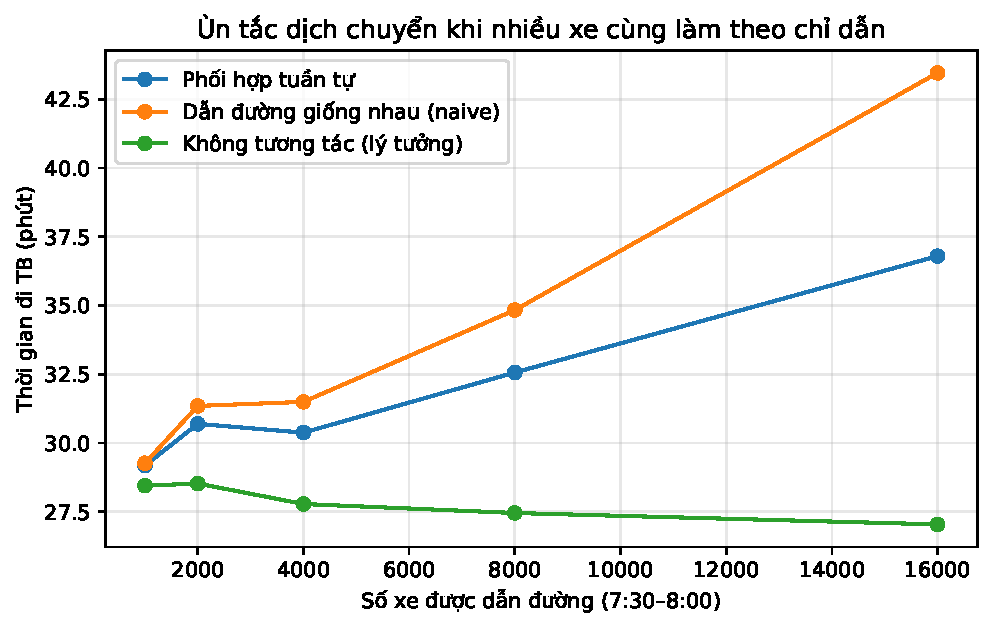
\includegraphics[width=0.66\linewidth]{multiagent.pdf}
\caption{Thời gian đi trung bình theo số xe được dẫn đường cùng lúc.}
\label{fig:ma}
\end{figure}

\subsubsection{Khi nào phương pháp đề xuất tốt hơn, và tại sao}

\begin{enumerate}[label=(\arabic*)]
    \item \textbf{TD-A* thay cho tuyến tĩnh} luôn có lợi khi vận tốc biến thiên theo giờ: regret giảm từ \DijRegret\% xuống
    \PoRegret\%. Lợi ích tương đối nhỏ hơn vào cao điểm vì trong mô hình mọi trục đều tắc.
    \item \textbf{Replan} có lợi khi dự báo sai cục bộ và lớn (sự cố, nhiễu cao); khi dự báo tốt, plan-once đã gần tối ưu.
    \textbf{Replan lười} cho cùng chất lượng và nhanh gấp \LazySpeedup{} lần; \textbf{D* Lite} nhanh hơn nhưng dùng chi phí
    snapshot nên có thể lệch nhẹ --- trên đồ thị cỡ này mọi biến thể đều đủ nhanh cho ứng dụng tương tác.
    \item \textbf{Dự báo GCN} có lợi khi nhiễu có tương quan không gian--thời gian và có mạng cảm biến: replan + GCN là phương
    pháp tốt nhất (\RpGnnRegret\%), và lợi ích tăng theo mức nhiễu. Với nhiễu độc lập, không có gì để lan truyền.
    \item \textbf{Định tuyến P90} không có lợi trong mô phỏng này do ước lượng phân vị từ ít mẫu và các ứng viên có rủi ro gần
    nhau; cần ngân hàng kịch bản lớn hơn hoặc mô hình rủi ro có cấu trúc.
    \item \textbf{RL} chỉ tiến gần được tìm kiếm khi được cung cấp thêm cấu trúc: thông tin toàn cục (cost-to-go), quan sát
    nhiều bước kết hợp học bắt chước, hoặc giao phần tìm đường cho TD-A* (RL lai). RL chọn từng cạnh với quan sát cục bộ không
    bảo đảm tới đích và còn kém một heuristic thủ công; RL lai bảo đảm tới đích nhưng chưa vượt replan. RL có thể có lợi khi
    không có mô hình chuyển trạng thái tường minh, khi mô hình sai lệch có hệ thống mà dữ liệu trải nghiệm phản ánh được, hoặc
    ở các quyết định cấp cao --- những điều kiện không có trong mô phỏng hiện tại.
\end{enumerate}
